

\documentclass[a4paper, 10pt, spanish]{article}
\usepackage{color}
\definecolor{cadet}{rgb}{0.33, 0.41, 0.47}
\definecolor{orange}{rgb}{0.93, 0.53, 0.18}
\definecolor{carminered}{rgb}{1.0, 0.0, 0.22}
\definecolor{green}{rgb}{0.33, 0.42, 0.18}
\definecolor{darkmagenta}{rgb}{0.55, 0.0, 0.55}
\usepackage{anysize}
\usepackage{amsmath}
\usepackage{biblatex}
\usepackage{float}
\usepackage{array} % 1
\usepackage{graphicx}
\usepackage{tikz}
\usetikzlibrary{calc,patterns,angles,quotes}
\usetikzlibrary{calc,decorations.pathmorphing,patterns}
\usepackage{graphicx}
\usepackage[spanish]{babel}
\usepackage[T1]{fontenc}
\usepackage[utf8]{inputenc}
\usepackage{textcomp}
\usepackage{fancyhdr}
\usepackage{color}
\usepackage{courier}
\usepackage{multirow}
\usepackage{float}
\usepackage{listings}
\usepackage{pgfplots,filecontents}
\pgfplotsset{compat=1.7}
\pgfplotsset{compat=newest}
\usepgfplotslibrary{units}
\usepackage[siunitx]{circuitikz}
\usepackage{caption}
\usepackage{subcaption}
\usepackage{cleveref}
\usepackage{tabularx}
\usepackage{lscape}
\usepackage{pdflscape}
\usepackage{booktabs}


\usepackage{lastpage}   % Para poder saber cuántas páginas tiene el documento
\pagestyle{fancy}
\renewcommand{\sectionmark}[1]{\markboth{}{\thesection\ \ #1}}
\fancyhead{}	% Elimino el contenido del encabezado
% El siguiente texto a la derecha (izquierda) en páginas pares (impares)
\fancyhead[RE,LO]{86.06 - Circuitos Electrónicos - Informe N\textsuperscript{o}2}
\fancyhead[R]{FIUBA}

\fancyfoot{}	% Elimino el contenido del pie de página
% A la izquierda (derecha) en páginas pares (impares): nro. de página / total
\fancyfoot[LE,RO]{\thepage/\pageref{LastPage}}



\begin{document}


\marginsize{2cm}{2cm}{2cm}{2cm}
%
% Carátula:
%
\begin{titlepage}

\thispagestyle{empty}

\begin{center}

\includegraphics[scale=0.3]{fiuba.pdf}\\
\large{\textsc{Universidad de Buenos Aires}}\\
\large{\textsc{Facultad de Ingeniería}}\\
% Modificar año y cuatrimestre
\small{Año 2019 - 2\textsuperscript{o} cuatrimestre}
\end{center}

\vfill

\begin{center} % Modificar el código de ser necesario
\Large{\underline{\textsc{Circuitos Electrónicos (86.06)}}}\\ \vspace{0.5cm}
\Large{\underline{\textsc{Etapas con Transistores Discretos}}}\\ \vspace{0.5cm}
\Large{\underline{\textsc{Informe de Laboratorio N\textsuperscript{o}~2}}}
\end{center}

\vfill

\begin{center}
\large{José F. González - 100063 - \footnotesize{\verb!<jfgonzalez@fi.uba.ar>!}}\\ \vspace{0.25cm}
\large{Gottfried, Joel - 102498 - \footnotesize{\verb!<joelgottfried99@gmail.com>!}}\\\vspace{0.25cm}
\large{Urquiza, Elias - 100714 - \footnotesize{\verb!<eurquiza@fi.uba.ar>!}}\\
\end{center}

\vfill

\hrule
\vspace{0.2cm}

% Modificar código de ser necesario
\noindent\small{86.06 - Circuitos Electrónicos \hfill }

\end{titlepage}

%
% Hago que las páginas se comiencen a contar a partir de aquí:
%
\setcounter{page}{1}

%
% Pongo el índice en una página aparte:
%
\tableofcontents
\newpage


\section{Especificaciones}

Necesitamos diseñar una etapa amplificadora con un transistor \textbf{JFET 2N5486} donde la ganancia de potencia sea $G_p > 100$.

\section{Diseño de la Etapa Amplificadora}

Para la elección de la tecnología del transistor se tuvo en cuenta que al necesitar la etapa una alta ganancia de potencia esta será fácil de obtener si el dispositivo tiene corrientes de entrada casi nulas dando ganancias de corriente muy elevadas. Luego se decidió utilizar transistores FET que cumplen esta característica. En particular utilizamos JFET para familiarizarnos con su funcionamiento. En cuanto a la configuración en que funciona el transistor tenemos tres posibilidades, utilizarlo como Gate común, Drain común o Source común. El primer caso se descartó siendo que la configuración Gate Común tiene una ganancia de corriente unitaria \textit{(current buffer)}. El Drain Común se descarta pues tiene ganancia de tensión casi unitaria \textit{(seguidor por source)}. Finalmente usamos la opción de Source Común que nos permite controlar tanto la ganancia de tensión como la de corriente.

 \begin{figure}[h]
                                            \centering
                                            \begin{circuitikz}
                                         \draw
                                          % Drawing a npn transistor
                                          (0,0) node[njfet](fet){} node[left=0.5cm]{2N5486}
                                          (fet.G) -- ++ (0,0) to[short] ++(-2,0) node (RG) {} to[R]  ++(0,-2.5) node[ground] {}; \draw (RG) ++(0.5cm,-0.5cm) node[]{$R_G$};
                                          \draw
                                          (RG) -- ++ (0,0) node(CA1){} to[C] ++(-2,0) node(Rs) {} to[R] ++(-2.5,0) to[short,-o] ++(0,0);\draw (CA1)++(-1cm,0.75cm) node {$C_{A1}$};
                                          \draw (Rs) ++(-1.5cm,0.5cm) node {$R_s$};
                                          \draw
                                          (fet.S) -- ++ (0,0) node[right] {$R_S$} to[R] ++(0,-2) node[ground] {};
                                          \draw
                                          (fet.D) -- ++ (0,0) to[R] ++(0,2.5) node(RD){} to[short,-o] ++(0,0); \draw (RD) ++(0,-0.25cm) node[right] {$R_D$}; \draw (RD) node[above] {$V_{DD}$};
                                          \draw
                                          (fet.D) -- ++(0,0) node(CA2){} to[C] ++(5,0) node(RL){} to[R] ++(0,-3.5) node[ground] {}; \draw (RL) ++(0.5cm,-1cm) node[]{$R_L$}; \draw (CA2) ++(2.5cm,0.75cm) node{$C_{A2}$};


                                          %%TENSIONES Y CORRIENTES
                                          \draw (Rs) ++(-2cm,-0.75cm) [-latex, thick, red] -- ++(1.5cm,0) node[above] {$i_s$};
                                          \draw (Rs) ++ (-2.5,-3) [-latex,thick,blue] -- ++ (0,2.75) node[left] {$v_s$};
                                          \draw (fet.G) ++(-1.5,0.75) [-latex,red,thick] -- ++(1.5,0) node[above] {$i_G$};
                                          \draw (RL) ++ (0,0.75) [-latex, red, thick] -- ++ (-1.5,0) node[above] {$i_o$};
                                          \draw (RL) ++ (1,-3) [-latex, blue, thick] -- ++ (0,2.5) node [right] {$v_o$};
                                            \end{circuitikz}
                                            \caption{Etapa Amplificadora - Source Común}
                                            \label{fig:circuito}
                                          \end{figure}



En la Figura \ref{fig:circuito} se muestra el circuito propuesto que consiste en un JFET Canal N en modo Source Común con una camino de realimentación. Para este circuito definimos la ganancia de potencia para señales senoidales como

\begin{equation}
	G_P = \frac{P_O}{P_I} = \frac{\hat{V_O}\hat{I_O}/2}{\hat{V_S}\hat{I_S}/2} = \frac{\hat{V_O}\hat{I_O}}{\hat{V_S}\hat{I_S}} = A_{vs}\cdot A_{i}
	\end{equation}

De la hoja de datos\footnote{https://www.mouser.com/datasheet/2/68/2n5484-5486-51207.pdf} se obtienen los datos para definir una \textbf{zona de operación segura} de la Figura \ref{fig:zona_segura} dentro de los cuales podremos polarizar al transistor.



\begin{figure}[h]
    \begin{center}
      \begin{tikzpicture}[scale=0.9]
      \draw [-latex] (0,0) -- (5.5,0) node [above] {$V_{DS}$};
      \draw [-latex] (0,0) -- (0,5.5) node [above] {$I_{D}$};
      \draw [red,thick] (4.8,1.2) -- (4.8,0) node[below] {$25\ V$};
      \draw [red,thick] (2.06,4.8) -- (0,4.8) node[left] {$30\ mA$};
      \draw [red,thick] (4.8,1.2) parabola (2.06,4.8);
      \draw [red,dashed] (2.06,4.8) -- (2.06,0) node[below] {$10,3\ V$};
      \draw [red,dashed] (4.8,1.2) -- (0,1.2) node[left] {$12.4\ mA$};
      \end{tikzpicture}
      \begin{tikzpicture}[scale=0.9]
      \draw [-latex] (0,0) -- (5.5,0) node [above] {$V_{DS}$};
      \draw [-latex] (0,0) -- (0,5.5) node [above] {$I_{D}$};
      \draw [thick, blue] (0,4.8) -- (3.6,0);
      \draw (0,4.8) node[left] {$I_{DQ} + \frac{V_{DSQ}}{R_{DA}+R_S}$};
      \draw [thick, green] (0,3.6) -- (5.3,0);
      \draw (5.3,0) node [below] {$V_{DD}$} ;
      \draw (0,3.6) node[left]{$\frac{V_{DD}}{R_D+R_S}$};
      \draw [dashed] (1.8,2.4) -- (0,2.4) node[left] {$I_{DQ}$};
      \draw [dashed] (1.8, 2.4) -- (1.8,0) node [below] {$V_{DSQ}$};
      \end{tikzpicture}

    \end{center}
    \caption{\textbf{Izquierda:} Zona de operación segura para el transistor. \textbf{Derecha:} Rectas de carga para el circuito propuesto.}
    \label{fig:zona_segura}
    \end{figure}


\newpage
\subsection{Rectas de Carga}


 \begin{figure}[h!]
                                            \centering
                                            \begin{circuitikz}
                                         \draw
                                          % Drawing a npn transistor
                                          (0,0) node[njfet](fet){} node[left=0.5cm]{2N5486}
                                          (fet.G) -- ++ (0,0) to[short] ++(-2,0) node (RG) {} to[R]  ++(0,-2.5) node[ground] {}; \draw (RG) ++(0.5cm,-0.5cm) node[]{$R_G$};
                                          \draw
                                          (fet.S) -- ++ (0,0) node[right] {$R_S$} to[R] ++(0,-2) node[ground] {};
                                          \draw
                                          (fet.D) -- ++ (0,0) to[R] ++(0,2.5) node(RD){} to[short,-o] ++(0,0); \draw (RD) ++(0,-0.25cm) node[right] {$R_D$}; \draw (RD) node[above] {$V_{DD}$};

                                            \end{circuitikz}
                                            \caption{Etapa Amplificadora - Circuito de continua}
                                            \label{fig:circuito_continua}
                                          \end{figure}

En la Figura \ref{fig:circuito_continua} se ve el circuito de continua, donde la recta de carga estática se obtiene al recorrer la malla de salida:

\begin{equation}
	I_D = \frac{V_{DD}}{R_D + R_S} - \frac{V_{DSQ}}{R_D + R_S}
	\end{equation}

y la recta de carga dinámica será

\begin{equation}
	i_D = \frac{-1}{(R_D//R_L) + R_S}\cdot v_{DS} + I_{DQ} + \frac{V_{DSQ}}{(R_D//R_L) + R_S}
	\end{equation}


\newpage
\subsection{Parámetros de pequeña señal}\label{sec:parametros}



 \begin{figure}[h!]
                                            \centering
                                            \begin{circuitikz}
                                         \draw
                                          % Drawing a npn transistor
                                          (0,0) node[njfet](fet){} node[left=0.5cm]{2N5486}
                                          (fet.G) -- ++ (0,0) to[short] ++(-2,0) node (RG) {} to[R]  ++(0,-2.5) node[ground] {};\draw (RG) ++(0.5cm,-0.5cm) node[]{$R_G$};
                                          \draw
                                          (RG) -- ++ (0,0) node(CA1){} to[short] ++(-2,0) node(Rs) {}to[R] ++(-2.5,0) to[short,-o] ++(0,0) node[left]{$v_s$};
                                          									\draw (Rs) ++(-1.5cm,0.5cm) node {$R_s$};
                                          \draw
                                          (fet.S) -- ++ (0,0) node[right] {$R_S$} to[R] ++(0,-2) node[ground] {};
                                          \draw
                                          (fet.D) -- ++ (2.5,0) node(RD){} to[R]  ++(0,-3.5) node[ground] {}; \draw (RD) ++(0.5cm,-1cm) node[]{$R_D$};
                                         \draw
                                          (fet.D) -- ++(0,0) to[short] ++(5,0) node(RL){} to[R] ++(0,-3.5) node[ground] {}; \draw (RL) ++(0.5cm,-1cm) node[]{$R_L$};

                                            \end{circuitikz}
                                            \caption{Etapa Amplificadora - Circuito de señal a frecuencias medias}
                                          \end{figure}




Del circuito de señal a frecuencias medias podemos obtener los siguientes parámetros por inspección, en una primera aproximación \textbf{despreciando efectos de segundo orden en el transistor}.
La ganancia de tensión será

\begin{equation}
A_v = \frac{v_o}{v_i} = \frac{-i_o(R_D // R_L)}{v_{gs}+ v_{R_S}} = \frac{-(R_D//R_L)}{\frac{v_{gs}}{i_o}+R_S} = \frac{-(R_D//R_L)}{\frac{1}{g_m}+R_S}
\end{equation}

que referida al generador resulta

\begin{equation}
A_{vs} = A_v \frac{v_i}{v_s} = A_v \frac{R_G}{R_G + R_s}
\end{equation}

La ganancia de corrientes será

\begin{equation}
A_i = \frac{i_o}{i_s} = \frac{i_o}{\frac{v_i}{R_G}} = \frac{i_o}{v_{gs}+i_o R_S} = \frac{R_G}{\frac{1}{g_m}+R_S}
\end{equation}

Asumiendo que se cumple que $R_S >> 1/g_m$ y $R_s << R_G$ \textbf{se puede expresar la ganancia de potencia en una primera aproximación que depende integramente de la elección de resistencias}

\begin{equation}
G_P = A_{vs}\times A_i \approx \frac{R_D//R_L}{R_S} \times \frac{R_G}{R_S}
\end{equation}


la resistencia de entrada y salida serán:

\begin{equation}
R_I = R_G
\end{equation}

\begin{equation}
R_O = R_D(1+g_mR_S)
\end{equation}


\subsection{Elección de valores}\label{sec:valores}

Con el objetivo de obtener $G_P > 100$ se eligieron los valores de resistencias y fuente de polarización del Cuadro \ref{tab:valores}. Para ello se utilizó la expresión aproximada de Ganancia de Potencia obtenida en la Sección \ref{sec:parametros} que se la evaluó en los distintos valores ofrecidos por el LACE. \textbf{La elección de resistores es tal que ,para la tensión de alimentación elegida, permita la mayor ganancia de potencia posible sin que el transistor se salga de saturación.}

\begin{table}[h]
\centering
\begin{tabularx}{0.7\textwidth}{XXXXX}
\hline
 $R_G$  		& $R_D$ 		& $R_S$ 			& $R_L$ 		& $V_{DD}$ \\
 \hline
 $820\ k\Omega$ & $1\ k\Omega$ 	& $470\ \Omega$ 	& $10\ k\Omega$ & $12\ V$ \\
\hline
\end{tabularx}
\caption{Valores propuestos para la etapa amplificadora.}
\label{tab:valores}
\end{table}



\subsection{Dispersión de parámetros}

En los Cuadros \ref{tab:dispersion} y \ref{tab:dispersion2} se muestran los distintos parámetros del amplificador y el punto de reposo para los valores extremos de los parámetros $I_{DSS}$ y $V_P$ del JFET con la elección de resistencias de la sección anterior.



\begin{table}[h]
\centering
\begin{tabularx}{1\textwidth}{XXXXXXXX}
\hline
\multicolumn{2}{c}{}				& \multicolumn{4}{c}{Parámetros del Amplificador}						& \multicolumn{2}{c}{Punto de Reposo} \\
									\cmidrule(r){3-6}														\cmidrule(r){7-8}
\multicolumn{2}{c}{$(I_{DSS},V_{P})$}& $|A_{vs}|$  		& $|A_{i}|$ 		& $G_P$ 			& $g_m$ 		& $I_{DQ}$ 			& $V_{DSQ}$			\\
\cmidrule(r){1-2}  									\cmidrule(r){3-3} \cmidrule(r){4-4} 	\cmidrule(r){5-5} 	\cmidrule(r){6-6} \cmidrule(r){7-7} 	\cmidrule(r){8-8}
\multicolumn{2}{c}{$(20\ mA,-6\ V)$}& $1.2$	& $1096$	& $1316$ & $3.6\ mA/V$ & $5.8\ mA$& $3.5\ V$\\
\hline
\multicolumn{2}{c}{$(14\ mA,-4\ V)$}& $1.2$	& $1108$	& $1329$ & $3.7\ mA/V$& $3.9\ mA$ & $6.3\ V$\\
\hline
\multicolumn{2}{c}{$$(8\ mA,-2\ V)$$}&$1.3$	& $1139$	& $1480$ & 4\ mA/V & $2\ mA$ & $9.1\ V$ \\
\hline
\hline
\multicolumn{2}{c}{\textcolor{red}{Dispersión:}} & $8\%$ & $3\%$ & $13\%$ & $11\%$ & $190\%$ & $160\% $\\
\hline
\end{tabularx}
\caption{Parámetros teóricos de la etapa amplificadora.}
\label{tab:dispersion}
\end{table}


\begin{table}[h]
\centering
\begin{tabularx}{0.5\textwidth}{XXXX}
\hline
\multicolumn{2}{c}{}				& \multicolumn{2}{c}{Parámetros del Amplificador}					 \\
									\cmidrule(r){3-4}
\multicolumn{2}{c}{$(I_{DSS},V_{P})$}& $R_I\ (k\Omega)$  		& $R_O\ (k\Omega)$ 				\\
\cmidrule(r){1-2}  									\cmidrule(r){3-3} \cmidrule(r){4-4}
\multicolumn{2}{c}{$(20\ mA,-6\ V)$}& $820$	& $2.7$	\\
\hline
\multicolumn{2}{c}{$(14\ mA,-4\ V)$}& $820$	& $2.7$	\\
\hline
\multicolumn{2}{c}{$$(8\ mA,-2\ V)$$}&$820$	& $2.9$	\\
\hline
\hline
\multicolumn{2}{c}{\textcolor{red}{Dispersión:}} & $0\%$ & $7\%$ \\
\hline
\end{tabularx}
\caption{Parámetros teóricos de la etapa amplificadora - Continuación.}
\label{tab:dispersion2}
\end{table}

Para obtener estos valores se tuvieron en cuenta los siguientes puntos

\begin{itemize}
	\item En ningún caso se cumple $1/g_m << R_S$ luego se usaron las expresiones completas de ganancias.
	\item Se despreciaron efectos de segundo orden en el transistor.
	\item Se utilizó para describir la dispersión el rango porcentual respecto al mínimo dado por
		\begin{equation}
		\delta f \% = \frac{f_{MAX}-f_{MIN}}{f_{MIN}}\times 100 \nonumber
		\end{equation}
	\item Se asumieron valores típicos como los valores promedios a falta de esta información en hoja de datos.
	\item Se despreciaron corrientes de Gate.
	\end{itemize}


En la Figura \ref{fig:dispersion} se muestran los distintos puntos de reposo en el contorno de la zona segura.


\begin{figure}[h]
    \begin{center}
      \begin{tikzpicture}[scale=0.5]
      \draw [-latex] (0,0) -- (15,0) node [above] {$V_{DS}\ (V)$};
      \draw [-latex] (0,0) -- (0,10) node [above] {$I_{D}\ (mA)$};

      %%RCE
      \draw [thick] (0,8.2) node[left] {$8.2$} -- (12,0) node[below]{$12\ V$};

      \draw [fill] (3.5,5.8) circle (0.15);
      \draw [fill] (6.3,3.9) circle (0.15)
      		[thick, blue] (0,8.5) node[right]{RCD}-- (11.7,0);
      \draw [fill] (9.1,2) circle (0.15);


      \draw [dashed] (6.3,3.9) -- (6.3,0) node[below]{$6.3$} -- (6.3,-8);
      \draw [thick,blue,] (6.3,0) [rotate=90]sin (4.3,-5) cos (2.3,0) sin (0.3,+5) cos (-1.7,0);
      \draw [latex-,-latex] (6.3,-4) -- (11.7,-4); \draw (9.3,-4) node[below]{$v_o$};

      \end{tikzpicture}

    \end{center}
    \caption{Recta de carga estática con puntos de reposo extremos y típico.}
    \label{fig:dispersion}
    \end{figure}



\subsection{Realimentación en señal}

\textbf{El circuito presenta un camino de realimentación de señal de muestro de corriente suma de tensión.} En la Figura \ref{fig:realimentacion} se hace un análisis de incrementos para mostrar que la realimentación es negativa.


 \begin{figure}[h!]
                                            \centering
                                            \begin{circuitikz}
                                         \draw
                                          % Drawing a npn transistor
                                          (0,0) node[njfet](fet){} node[left=0.5cm]{2N5486}
                                          (fet.G) -- ++ (0,0) to[short] ++(-2,0) node (RG) {} to[R]  ++(0,-2.5) node[ground] {};\draw (RG) ++(0.5cm,-0.5cm) node[]{$R_G$};
                                          \draw
                                          (RG) -- ++ (0,0) node(CA1){} to[short] ++(-2,0) node(Rs) {}to[R] ++(-2.5,0) to[short,-o] ++(0,0) node[left]{$v_s$};
                                          									\draw (Rs) ++(-1.5cm,0.5cm) node {$R_s$};
                                          \draw
                                          (fet.S) -- ++ (0,0) node[right] {$R_S$} to[R] ++(0,-2) node[ground] {};
                                          \draw
                                          (fet.D) -- ++ (2.5,0) node(RD){} to[R]  ++(0,-3.5) node[ground] {}; \draw (RD) ++(0.5cm,-1cm) node[]{$R_D$};
                                         \draw
                                          (fet.D) -- ++(0,0) to[short] ++(5,0) node(RL){} to[R] ++(0,-3.5) node[ground] {}; \draw (RL) ++(0.5cm,-1cm) node[]{$R_L$};


                                         %%% CORRIENTES y TENSIONES

                                         \draw (fet.D) [red,-latex] ++(1cm,0.5cm) node[above] {$i_o \uparrow\  \Rightarrow i_o \downarrow \downarrow$} to[short] ++(-1cm,0);

                                         \draw (fet.S) ++(0.75cm,-2cm) [blue,-latex] parabola ++(0cm,2cm) node[right]{$v_{rs} \uparrow$} ;

                                         \draw (fet.S) ++(-0.25cm,-0.25cm) [blue,-latex] parabola ++(-1cm,0.5cm) node[left] {$v_{gs} \downarrow$};
                                            \end{circuitikz}
                                            \caption{Análisis de incrementos de la realimentación}
                                            \label{fig:realimentacion}
                                          \end{figure}


De las expresiones de ganancia de tensión podemos obtener que el \textbf{factor de realimentación} para este circuito es
\begin{equation}
	FR = 1+g_mR_S
	\end{equation}

\subsection{Señales sin recorte}\label{sec:distorsiones}

Asumiendo el punto de operación Q asociado a los valores típicos del transistor $I_{DSS} = 14\ mA$ y $V_P = -4\ V$ obtenemos las máximas señales sin distorsión. De la Figura \ref{fig:dispersion} se ve que para los valores típicos la máxima tensión a la salida sin distorsión por recorte ni triodo serán de tensión máxima aproximadamente $\hat{v_o} = 6\ V$. Luego, en este punto la ganancia referida al generador es de unos $A_{vs} = 1.2$, entonces la máxima tensión que podemos poner del generador, a valores típicos, será

\begin{equation}
	v_s = \frac{v_o}{A_{vs}} \approx 5\ V \nonumber
	\end{equation}

\textbf{El límite por alinealidad será el determinante de las máximas señales del generador}. Aceptando un error del $10\ \%$ en la linealización se obtiene una cota de $v_{gs} < 25\ mV$ asociado a la tensión térmica.

\begin{equation}
	v_{gs} = 25\ mV \Rightarrow v_o = -i_o\times R_D//R_L = -g_m\cdot v_{gs} \times R_D//R_L = - 80\ mV \Rightarrow v_s = 67\ mV
	\end{equation}

\textbf{La máxima amplitud pico de señal que puede tener el generador sin distorsión de ningún tipo es $v_s = 67\ mV$ (cuando $I_{DSS} = 14\ mA$ y $V_P = -4\ V$).}


\subsection{Propagación de Errores}

\textbf{Los valores de resistencias poseen un error inherente de $\pm 5 \%$}. La dispersión de los distintos parámetros del amplificador nos da una idea de los extremos dentro del cuál podemos hallar esos valores mientras que para las mediciones vamos a querer ver que error se arrastra al usar las distintas ecuaciones obtenidas por inspección en la Sección \ref{sec:parametros}. Se utiliza la propagación de incertezas analítica para una función de N variables aleatorias $y=f(X_1,..,X_n)$ de valores medios $\mu_{X1},...,\mu_{XN}$ y varianza $\sigma_{X1}^2,...,\sigma_{XN}^2$

\begin{equation}
	\sigma_y^2 = \sum_{i}^{} (\frac{\delta y}{\delta x} \rvert_{\mu_{X1},..,\mu_{XN}})^2 \times \sigma_{Xi}^2 \nonumber
	\end{equation}

\subsubsection{Propagación en Ganancia de Tensión}

Obtuvimos para la ganancia de tensión referida al generador la expresión aproximada
\begin{equation}
	A_{vs} \approx \frac{-(R_D//R_L)}{R_S} \nonumber
	\end{equation}

La propagación resulta

\begin{equation}
	\delta^2 A_{vs} = (\frac{R_L^2}{R_S(R_D+R_L)^2})^2 \times \delta^2 R_D + (\frac{R_D^2}{R_S(R_D+R_L)^2})^2 \times \delta^2R_L + (\frac{R_D//R_L}{R_S^2})^2\times \delta^2R_S \nonumber
	\end{equation}

que evaluado en la elección de resistencias (valores medios) de la Sección \ref{sec:valores} con desviación estandar $\delta R = 5\% \mu_R$ se obtiene una desciación estandar

\begin{equation}
	\delta A_{vs} \approx 2 \nonumber
	\end{equation}

donde el término que más pesa es la incerteza en $R_L$.


\subsubsection{Propagación en Ganancia de Corriente}

Se obtuvo la aproximación para la ganancia de corriente

\begin{equation}
	A_i = \frac{R_G}{R_S} \nonumber
	\end{equation}

la propagación de incertezas resulta

\begin{equation}
	\delta^2 A_i = (\frac{1}{R_S})^2 \times \delta^2 R_G + (\frac{R_G}{R_S^2})^2 \times \delta^2 R_S \nonumber
	\end{equation}

evaluando en los valores medios y desviaciones

\begin{equation}
	\delta A_i \approx 98 \nonumber
	\end{equation}




\subsubsection{Propagación en Ganancia de Potencia}

Siendo por definición $G_P = A_{vs}\times A_{i}$ propagamos errores como

\begin{equation}
	\delta G_P = \sqrt{A_i^2 \times \delta^2 A_{vs} + A_{vs}^2\times \delta^2A_i} \nonumber
	\end{equation}

que para los valores obtenidos en las mediciones (ver Sección \ref{sec:mediciones}) vale

\begin{equation}
	\delta G_P \approx 1800 \nonumber
	\end{equation}


\subsubsection{Propagación en Resistencias de Entrada y Salida}

Para la resistencia de entrada la propagación es simplemente

\begin{equation}
	\delta R_I = \delta R_G = 0.005\cdot 820\ k\Omega = 4.1\ k\Omega \nonumber
	\end{equation}

Y en la Resistencia de Salida

\begin{equation}
	\delta^2 R_O = (1+g_mR_S)^2 \times \delta^2 R_D + (R_D\cdot g_m)^2 \times \delta^2 R_S + (R_DR_S)^2 \times \delta^2 g_m \nonumber
	\end{equation}

para simplificar asumimos $\delta^2 g_m = 39\ nS$ (estimación en base a valores típicos) para obtener

\begin{equation}
	\delta R_O \approx 162 \nonumber
\end{equation}


\newpage

\section{Mediciones}\label{sec:mediciones}

Se implementó el circuito de la Figura \ref{fig:circuito} en la placa provista por el LACE utilizando los valores de componentes y alimentaciones definidos en el Cuadro \ref{tab:valores}. Sobre la placa se midieron los parámetros del circuito amplificador que se resumen en el Cuadro \ref{tab:mediciones}. Para las señales de generador y de prueba se tuvo en cuenta el análisis de distorciones hecho en la Sección \ref{sec:distorsiones} y se usaron señales de $40\ mV$ pico a $1\ kHz$.


\begin{table}[h]
\centering
\begin{tabularx}{0.9\textwidth}{XXXXXXXX}
\hline
\multicolumn{1}{c}{}				& \multicolumn{5}{c}{Parámetros Medidos del Amplificador}						& \multicolumn{2}{c}{Punto de Reposo Medido} \\
									\cmidrule(r){2-6}														\cmidrule(r){7-8}
\multicolumn{1}{c}{}				& $|A_{vs}|$  		& $|A_{i}|$ 		& $G_P$ 			& $R_I\ (k\Omega)$ & $R_O\ (k\Omega)$ 		& $I_{DQ}$ 			& $V_{DSQ}$			\\
									\cmidrule(r){2-2} \cmidrule(r){3-3} \cmidrule(r){4-4} 	\cmidrule(r){5-5} 	\cmidrule(r){6-6} \cmidrule(r){7-7} 	\cmidrule(r){8-8}
\multicolumn{1}{c}{}				& $1.4 \pm 2$	& $917 \pm 98$	& $1284 \pm 1800$ & $820 \pm 4 $ & $1 \pm 0.162 $ & $5.80mA$& $3.5V$\\
\hline
\end{tabularx}
\caption{Parámetros medidos de la etapa amplificadora.}
\label{tab:mediciones}
\end{table}



\subsection{Ganancia de Tensión}



Para la medición de ganancia de tensión que fue definida como $A_{vs} = v_o/v_s$ se utilizó el banco de medición de la Figura \ref{fig:avs}. Donde se determina la ganancia inderectamente como el cociente de los valores pico a pico de las señales de entrada y salida.




\subsection{Ganancia de corriente}

La ganancia de corriente fue definida como $A_i = i_o/ i_s$. La corriente de salida $i_o$ se determina conociendo el valor $R_L$ como $i_o = v_o/R_L$ donde $v_o$ se obtuvo en la medición anterior de ganancia de tensión.


La corriente del generador se obtiene asumiendo que por el gate no circula corriente $i_G = 0$ y midiendo la señal de tensión sobre $R_G$ como muestra la Figura \ref{fig:avi} se determina como $i_s = v_{RG}/R_G$. En el Cuadro \ref{tab:mediciones} se muestran los resultados de esta medición.

\subsection{Resistencia de Salida}

Para medir la resistencia de salida se utilizó un divisor resistivo como el que se muestra en la Figura \ref{fig:ro}. Conociendo la tensión sobre la resistencia de prueba obtenemos
\begin{equation}
	i_p = \frac{v_{CH2}-v_{CH1}}{1\ k\Omega} \Rightarrow R_o + 1\ k\Omega = \frac{v_p}{i_p} = \frac{v_p}{v_{CH2}-v_{CH1}}1\ k\Omega
	\end{equation}
En el Cuadro \ref{tab:mediciones} se muestran los resultados de esta medición.

\subsection{Resistencia de Entrada}

Para medir la resistencia de entrada se utilizo la configuración de la Figura \ref{fig:ri} asumiendo $i_G = 0$ se obtiene la corriente de prueba como $v_{RG}/R_G = v_{CH1}/R_G$.
En el Cuadro \ref{tab:mediciones} se muestran los resultados de esta medición.



 \begin{figure}[htb]
                                            \centering
                                            \begin{circuitikz}[scale=0.8]
                                         \draw
                                          % Drawing a npn transistor
                                          (0,0) node[njfet](fet){} node[left=0.5cm]{2N5486}
                                          (fet.G) -- ++ (0,0) to[short] ++(-2,0) node (RG) {} to[R]  ++(0,-2.5) node[ground] {}; \draw (RG) ++(0.5cm,-0.5cm) node[]{$R_G$};
                                          \draw
                                          (RG) -- ++ (0,0) node(CA1){} to[C] ++(-2,0) node(Rs) {} to[R] ++(-2.5,0) to[short,-o] ++(0,0) node[left] (vs) {$v_s$} ;\draw (CA1)++(-1cm,0.75cm) node {$C_{A1}$};
                                          \draw (Rs) ++(-1.5cm,0.5cm) node {$R_s$};
                                          \draw
                                          (fet.S) -- ++ (0,0) node[right] {$R_S$} to[R] ++(0,-2) node[ground] {};
                                          \draw
                                          (fet.D) -- ++ (0,0) to[R] ++(0,2.5) node(RD){} to[short,-o] ++(0,0); \draw (RD) ++(0,-0.25cm) node[right] {$R_D$}; \draw (RD) node[above] {$V_{DD}$};
                                          \draw
                                          (fet.D) -- ++(0,0) node(CA2){} to[C] ++(5,0) node(RL){} to[R] ++(0,-3.5) node[ground] {}; \draw (RL) ++(0.5cm,-1cm) node[]{$R_L$}; \draw (CA2) ++(2.5cm,0.75cm) node{$C_{A2}$};

                                          %MED

                                          \draw (vs) ++ (0,2)  [-latex,thick , blue] node[above] {CH2} -- ++(0,-1.8);
                                          \draw (RL) ++ (0,2)  [-latex,thick , blue] node[above] {CH1} -- ++(0,-1.8);

                                            \end{circuitikz}
                                            \caption{Banco de medición - Ganancia de tensión}
                                            \label{fig:avs}
                                          \end{figure}


 \begin{figure}[htb]
                                            \centering
                                            \begin{circuitikz}[scale=0.8]
                                         \draw
                                          % Drawing a npn transistor
                                          (0,0) node[njfet](fet){} node[left=0.5cm]{2N5486}
                                          (fet.G) -- ++ (0,0) to[short] ++(-2,0) node (RG) {} to[R]  ++(0,-2.5) node[ground] {}; \draw (RG) ++(0.5cm,-0.5cm) node[]{$R_G$};
                                          \draw
                                          (RG) -- ++ (0,0) node(CA1){} to[C] ++(-2,0) node(Rs) {} to[R] ++(-2.5,0) to[short,-o] ++(0,0) node[left] (vs) {$v_s$} ;\draw (CA1)++(-1cm,0.75cm) node {$C_{A1}$};
                                          \draw (Rs) ++(-1.5cm,0.5cm) node {$R_s$};
                                          \draw
                                          (fet.S) -- ++ (0,0) node[right] {$R_S$} to[R] ++(0,-2) node[ground] {};
                                          \draw
                                          (fet.D) -- ++ (0,0) to[R] ++(0,2.5) node(RD){} to[short,-o] ++(0,0); \draw (RD) ++(0,-0.25cm) node[right] {$R_D$}; \draw (RD) node[above] {$V_{DD}$};
                                          \draw
                                          (fet.D) -- ++(0,0) node(CA2){} to[C] ++(5,0) node(RL){} to[R] ++(0,-3.5) node[ground] {}; \draw (RL) ++(0.5cm,-1cm) node[]{$R_L$}; \draw (CA2) ++(2.5cm,0.75cm) node{$C_{A2}$};

                                          %MED

                                          \draw (RG) ++ (0,2)  [-latex,thick , blue] node[above] {CH1} -- ++(0,-1.8);
                                          \draw (RL) ++ (0,2)  [-latex,thick , blue] node[above] {CH2} -- ++(0,-1.8);

                                            \end{circuitikz}
                                            \caption{Banco de medición - Ganancia de corriente}
                                            \label{fig:avi}
                                          \end{figure}


 \begin{figure}[htb]
                                            \centering
                                            \begin{circuitikz}[scale=0.8]
                                         \draw
                                          % Drawing a npn transistor
                                          (0,0) node[njfet](fet){} node[left=0.5cm]{2N5486}
                                          (fet.G) -- ++ (0,0) to[short] ++(-2,0) node (RG) {} to[R]  ++(0,-2.5) node[ground] {}; \draw (RG) ++(0.5cm,-0.5cm) node[]{$R_G$};
                                          \draw
                                          (RG) -- ++ (0,0) node(CA1){} to[C] ++(-2,0) node(Rs) {} to[R] ++(-2.5,0) to[short,-o] ++(0,0) node[left] (vs) {$v_s$} ;\draw (CA1)++(-1cm,0.75cm) node {$C_{A1}$};
                                          \draw (Rs) ++(-1.5cm,0.5cm) node {$R_s$};
                                          \draw
                                          (fet.S) -- ++ (0,0) node[right] {$R_S$} to[R] ++(0,-2) node[ground] {};
                                          \draw
                                          (fet.D) -- ++ (0,0) to[R] ++(0,2.5) node(RD){} to[short,-o] ++(0,0); \draw (RD) ++(0,-0.25cm) node[right] {$R_D$}; \draw (RD) node[above] {$V_{DD}$};
                                          \draw
                                          (fet.D) -- ++(0,0) node(CA2){} to[C] ++(2,0) node(Rx) {} to[R] ++(3,0) node(RL) {} to[american voltage source] ++(0,-3.5) node[ground] {}; \draw (RL) ++(0.5cm,-1cm) node[]{$v_p$}; \draw (CA2) ++(1cm,0.75cm) node{$C_{A2}$}; \draw (Rx) ++(1cm,0.5cm) node {$1\ k\Omega$};

                                          %MED

                                          \draw (Rx) ++ (0,2)  [-latex,thick , blue] node[above] {CH1} -- ++(0,-1.8);
                                          \draw (RL) ++ (0,2)  [-latex,thick , blue] node[above] {CH2} -- ++(0,-1.8);

                                            \end{circuitikz}
                                            \caption{Banco de medición - Resistencia de Salida}
                                            \label{fig:ro}
                                          \end{figure}





 \begin{figure}[ht]
                                            \centering
                                            \begin{circuitikz}[scale=0.8]
                                         \draw
                                          % Drawing a npn transistor
                                          (0,0) node[njfet](fet){} node[left=0.5cm]{2N5486}
                                          (fet.G) -- ++ (0,0) to[short] ++(-2,0) node (RG) {} to[R]  ++(0,-2.5) node[ground] {}; \draw (RG) ++(0.5cm,-0.5cm) node[]{$R_G$};
                                          \draw
                                          (RG) -- ++ (0,0) node(CA1){} to[C] ++(-2,0) node(Rs) {} to[R] ++(-2.5,0) to[american voltage source] ++(0,-2.5) node[ground] (G1) {} ;\draw (CA1)++(-1cm,0.75cm) node {$C_{A1}$}; \draw (G1) [thick,blue,-latex] ++(-0.75cm,0.25cm) -- ++(0,2cm) node[above] {$v_p$};
                                          \draw (Rs) ++(-1.5cm,0.5cm) node {$R_s$};
                                          \draw
                                          (fet.S) -- ++ (0,0) node[right] {$R_S$} to[R] ++(0,-2) node[ground] {};
                                          \draw
                                          (fet.D) -- ++ (0,0) to[R] ++(0,2.5) node(RD){} to[short,-o] ++(0,0); \draw (RD) ++(0,-0.25cm) node[right] {$R_D$}; \draw (RD) node[above] {$V_{DD}$};
                                          \draw
                                          (fet.D) -- ++(0,0) node(CA2){} to[C] ++(5,0) node(RL){} to[R] ++(0,-3.5) node[ground] {}; \draw (RL) ++(0.5cm,-1cm) node[]{$R_L$}; \draw (CA2) ++(2.5cm,0.75cm) node{$C_{A2}$};

                                          %MED

                                          \draw (RG) ++ (0,2)  [-latex,thick , blue] node[above] {CH1} -- ++(0,-1.8);


                                            \end{circuitikz}
                                            \caption{Banco de medición - Resistencia de Entrada}
                                            \label{fig:ri}
                                          \end{figure}

\clearpage

\section{Simulaciones}

\subsection{Rango de Frecuencias Medias}

Simulando la respuesta en frecuencia del circuito diseñado, se obtuvo la respuesta en frecuencia y se realizó un gráfico de bode del módulo y fase de la transferencia $V_o/V_i$ tal que se pudo concluir que, efectivamente, al trabajar con una frecuencia de señal de 1KHz nos encontraremos en frecuencias medias, donde se pueden despreciar los efectos reactivos del amplificador.
\begin{center}
  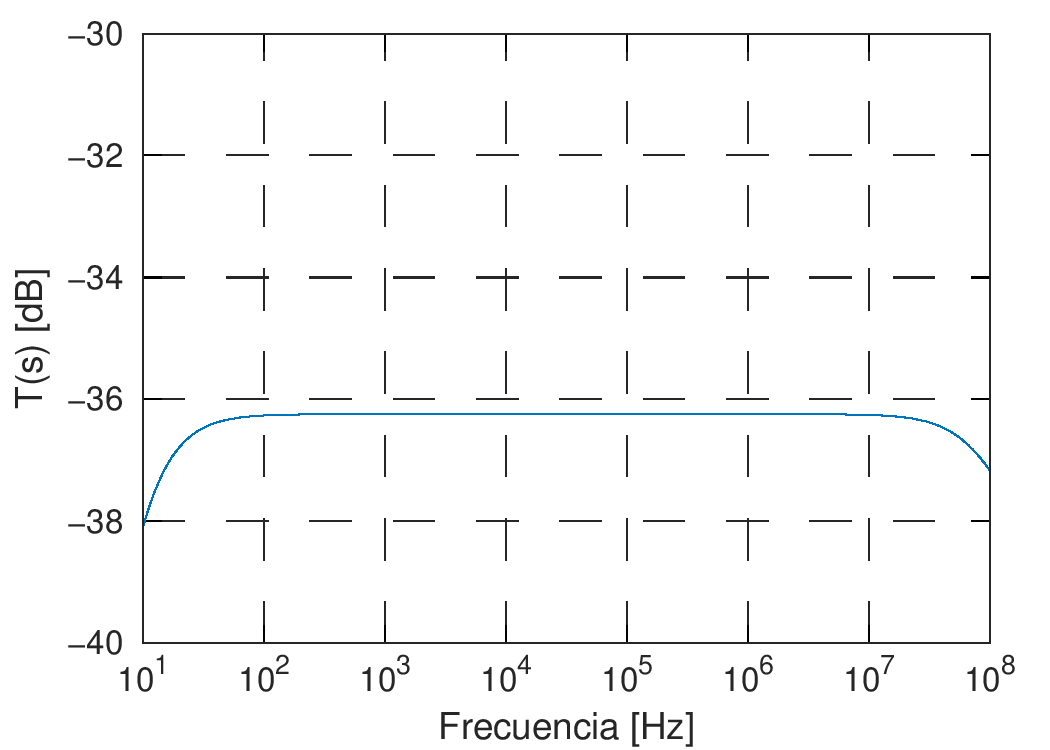
\includegraphics[width=0.5\textwidth]{bode-a-mod.png}
  \captionof{figure}{Respuesta en frecuencia del módulo de la transferencia.}
  \label{fig:amp-mod-bode}
\end{center}

\begin{center}
  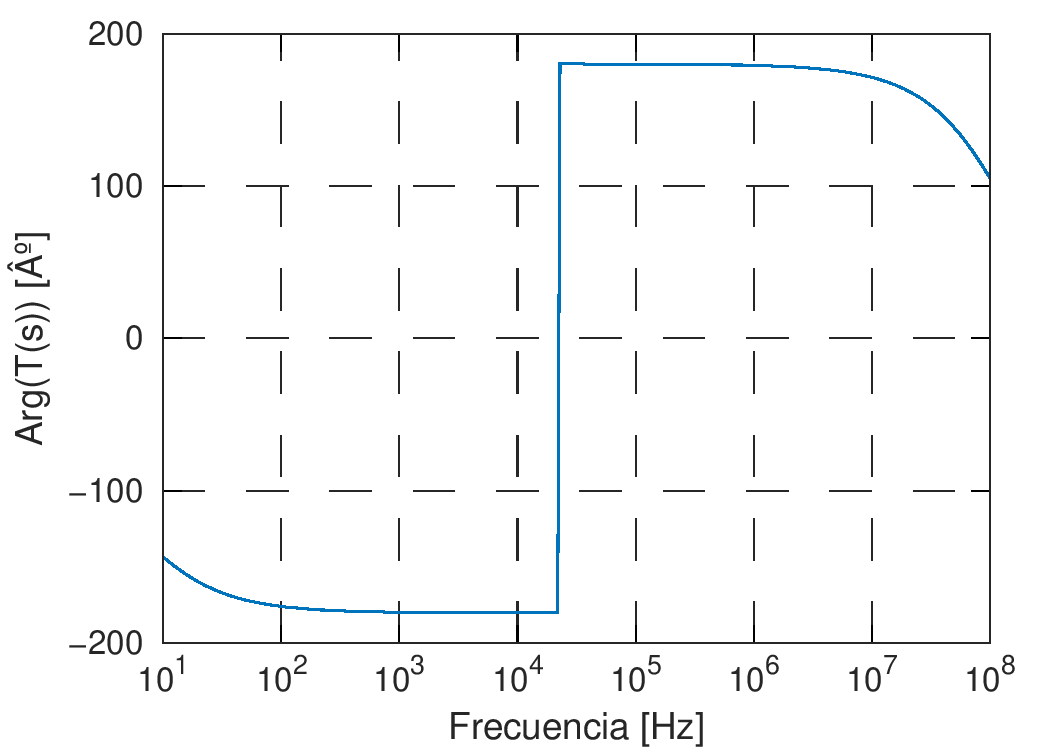
\includegraphics[width=0.5\textwidth]{bode-a-fase.png}
  \captionof{figure}{Respuesta en frecuencia de la fase de la transferencia.}
  \label{fig:amp-fase-bode}
\end{center}

\subsection{Resultados obtenidos}
Simulando las configuraciones presentadas en la sección 3, se obtuvieron los resultados del cuadro \ref{tab:simulaciones}.

\begin{table}[h]
\centering
\begin{tabularx}{0.9\textwidth}{XXXXXXXX}
\hline
\multicolumn{1}{c}{}				& \multicolumn{5}{c}{Parámetros Simulados del Amplificador}						& \multicolumn{2}{c}{Punto de Reposo Medido} \\
									\cmidrule(r){2-6}														\cmidrule(r){7-8}
\multicolumn{1}{c}{}				& $|A_{vs}|$  		& $|A_{i}|$ 		& $G_P$ 			& $R_I\ (k\Omega)$ & $R_O\ (k\Omega)$ 		& $I_{DQ}$ 			& $V_{DSQ}$			\\
									\cmidrule(r){2-2} \cmidrule(r){3-3} \cmidrule(r){4-4} 	\cmidrule(r){5-5} 	\cmidrule(r){6-6} \cmidrule(r){7-7} 	\cmidrule(r){8-8}
\multicolumn{1}{c}{}				& $1.5$	& $123.4$	& $190$ & $819$ & $0.995$ & $5.85mA$& $3.4V$\\
\hline
\end{tabularx}
\caption{Parámetros simulados de la etapa amplificadora.}
\label{tab:simulaciones}
\end{table}

Se puede observar que la ganancia de corriente es un $87\%$ menor a la presentada en el cuadro \ref{tab:mediciones}. Esto conlleva a una diferencia del $85\%$ en la ganancia de potencia. Consideramos que esto se debe a efectos no contemplados en los que la corriente consumida no es la que consideramos sobre la resistencia $R_G$.


\clearpage
        \section{Oscilador Senoidal por desplazamiento de fase}



 \begin{figure}[h!]
                                            \centering
                                            \begin{circuitikz}
                                         \draw
                                          % Drawing a npn transistor
                                          (0,0) node[npn](tbj){} node[right=0.5cm]{BC548B} ;
                                          \draw
                                          (tbj.B) to[short] ++(-2,0) node (A) {} to[R,*-] ++(0,-3) node[ground] {};
                                          \draw (A) ++(0.75cm,-0.75cm) node[] {$10\ k\Omega$};

                                          \draw (A) to[short] ++(0,0) to[C] ++(-2,0) node(B) {} to[C] ++(-2,0) node(C) {} to[C] ++(-2,0) node (D) {} to [short] ++(0,2) to [short,-o] ++ (12,0);
                                          \draw (B) to[R,*-] ++(0,-3) node[ground] {}; \draw (B) ++(0.75cm, -0.75cm) node {$10\ k\Omega$}; \draw (B) ++(0.75cm,0.75cm) node {$10\ nF$};

                                          \draw (C) to[R,*-] ++(0,-3) node[ground] {}; \draw (C) ++(0.75cm, -0.75cm) node {$10\ k\Omega$}; \draw (C) ++(0.75cm,0.75cm) node {$10\ nF$};

                                          \draw (D)  ++(0.75cm,0.75cm) node {$10\ nF$};


                                          \draw [dashed,red] (A) ++(0.5,0) -- ++(0,1.5) -- ++(-6,0) -- ++(0,-4.5) -- ++(6,0) -- ++(0,3);

                                          \draw (tbj.E) to[short,-*] ++ (0,-0.5) node(E) {} to [short] ++ (0.5,0) to[C] ++(0,-2) node[ground] {};
                                          \draw (E) to[short]  ++ (-0.5,0) to[R] ++(0,-2) node[ground] {}; \draw (E) ++(1cm,-0.5cm) node {$C$}; \draw (E) ++(-1.25cm,-0.5cm) node {$1\ k\Omega$};


                                          \draw (tbj.C) to[short,-*] ++(0,1.22) node(F) {} to[R,-o] ++ (0,2.5) node[above]{$V_{CC}$}; \draw (F) ++ (1cm, 1.5cm) node {$4.7\ k\Omega$};

                                          \draw (A) -- ++ (0,2.5) node(G){} to[R,-o] ++(0,2) node[above] {$V_{CC}$}; \draw (G) ++(1cm,1cm) node{$82\ k\Omega$};
                                            \end{circuitikz}
                                            \caption{Circuito Oscilador Senoidal por desplazamiento de fase.}
                                            \label{fig:oscilador}
                                          \end{figure}


        \subsection{Explicación Cualitativa}
        Para entender por qué la señal de salida $V_o$ es periódica cuasi senoidal, se puede realizar un análisis recorriendo el lazo de realimentación. Dada una perturbación en la señal presente en la base del transistor, que se considerará positiva, se puede esperar una señal negativa en la salida $V_o$. Es decir, existe un desfasaje de $180º$ entre la base y el colector. Esta señal de salida pasará por el bloque realimentador y, en un análisis simplificado, se puede considerar que el mismo está constituido por dos filtros RC pasa-altos idénticos y desacoplados entre sí, seguido por un capacitor de desacople antes de la malla de entrada. Dado que un filtro RC produce un desfasaje entre su entrada y su salida, es de esperarse que la señal que entregue a la base del transistor sea positiva -o negativa si la perturbación inicial es así-. Para que oscile, se requiere que dicho desfasaje total entre la entrada del bloque realimentador y su salida sea de $180º$ tal que se invierta completamente la señal $V_o$. En conclusión, se tiene una realimentación positiva.

        Aparte, para entender por qué la señal de salida $V_o$ es periódica cuasi senoidal, se puede recurrir a la forma exponencial de la Serie de Fourier, por la cual se tiene que la suma de infinitas exponenciales da lugar a una señal senoidal. En este caso, se tienen dos capacitores, para lo cual se tiene una suma de dos exponenciales y por ello se forma una señal cuasi-senoidal. De tener más bloques, teóricamente, se podría formar una señal senoidal más pura.

        La frecuencia de oscilación del circuito puede aproximarse según el desfasaje que aportará cada bloque RC. Se puede ver el diagrama de bode de fase de un pasa-altos en la figura \ref{fig:bode}. En la frecuencia de corte $f_c=\frac{1}{2\pi R C}$ se tiene un desfasaje de 45º, pero se requiere de uno de 90º para que los dos bloques desfasen 180º. Por lo tanto, se puede concluir que la frecuencia de oscilación estará por debajo de la de corte y se encontrará aproximadamente entre los 400Hz y 600Hz.

        \begin{center}
          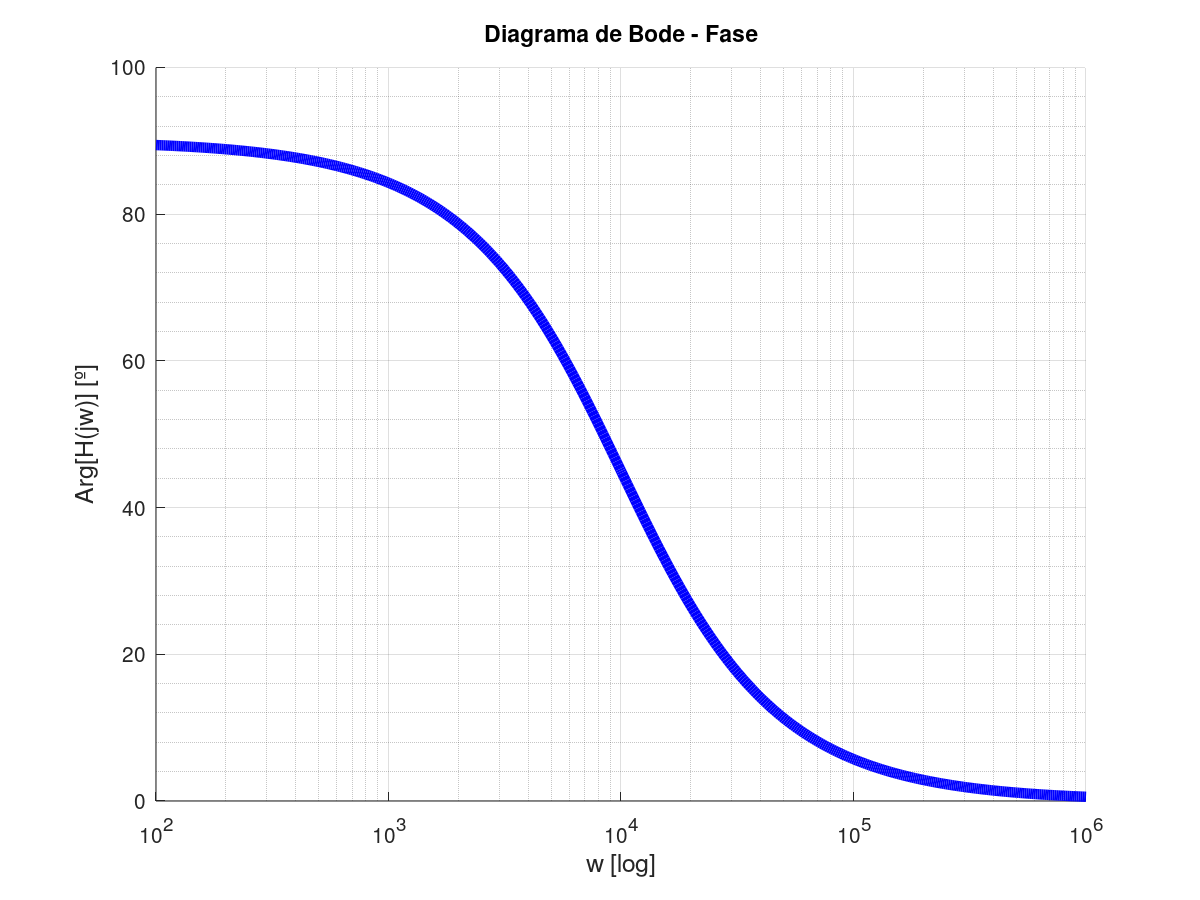
\includegraphics[width=0.6\textwidth]{bode-fase.png}
          \captionof{figure}{Diagrama de bode de fase para un RC pasa altos con $R=10K\Omega$ y $C=10nF$.}
          \label{fig:bode}
        \end{center}

        Para entender los rangos de tensión en que funciona el oscilador, es de utilidad observar la figura \ref{fig:rectas_carga_oscil}. Consideraremos que ambas rectas de carga coinciden, para simplificar el análisis. La oscilación del punto Q sobre la recta estará limitada por la diferencia de tensión entre el $V_{CQ}$ y $V_{CC}$. Esto es así ya que la carga y descarga de los capacitores del bloque de realimentación estará limitada por el régimen de corte, punto en el cual se realimenta positivamente un desplazamiento al otro extremo y, en caso de que se alcance, estará limitado también por el régimen de saturación. Si se disminuye $V_{CC}$, la recta se desplaza y el punto Q entra en corte, motivo por el cual dejará de oscilar el circuito.

        \begin{figure}[h]
            \begin{center}
              \begin{tikzpicture}[scale=0.9]
              \draw [-latex] (0,0) -- (5.5,0) node [above] {$V_{CE}$};
              \draw [-latex] (0,0) -- (0,5.5) node [above] {$I_{C}$};
              \draw [thick, blue] (0,4.8) -- (3.6,0);
              \draw (0,4.8) node[left] {$I_{CQ} + \frac{V_{CEQ}}{R_{ca}}$};
              \draw [thick, green] (0,3.6) -- (5.3,0);
              \draw (5.3,0) node [below] {$V_{CC}$} ;
              \draw (0,3.6) node[left]{$\frac{V_{C}}{R_C+R_E}$};
              \draw [dashed] (1.8,2.4) -- (0,2.4) node[left] {$I_{CQ}$};
              \draw [dashed] (1.8, 2.4) -- (1.8,0) node [below] {$V_{CEQ}$};
              \end{tikzpicture}
            \end{center}
      \caption{Rectas de Carga Estática y Dinámica del circuito de la fig. \ref{fig:oscilador}.}
      \label{fig:rectas_carga_oscil}
      \end{figure}

        \subsection{Medición y Simulación}
        Se obtuvo la figura \ref{fig:med_out_oscilador} al armar el circuito en el laboratorio. Se puede observar que \textbf{la frecuencia de oscilación es de 500Hz, y la señal de 14V pico-pico esta acoplada a una tensión continua de 13V. Se encontró también que la tensión $V_{CC}$ para la cual se detiene la oscilación es de aproximadamente 8V.}

        Por otro lado, al simular el circuito se obtuvo una señal de 515Hz con amplitud pico a pico de 13.7V acoplada a una señal continua de 13.03V, como se puede observar en la figura \ref{fig:sim_out_oscilador}. También se obtuvo la FFT de la señal de salida, presente en la figura \ref{fig:fft} y se puede observar que el armónico predominante es el de aproximadamente 500Hz, por lo que \textbf{se realizó un cálculo de la Distorsión Armónica Total y se obtuvo un valor de 14.24\%.}

        \begin{center}
          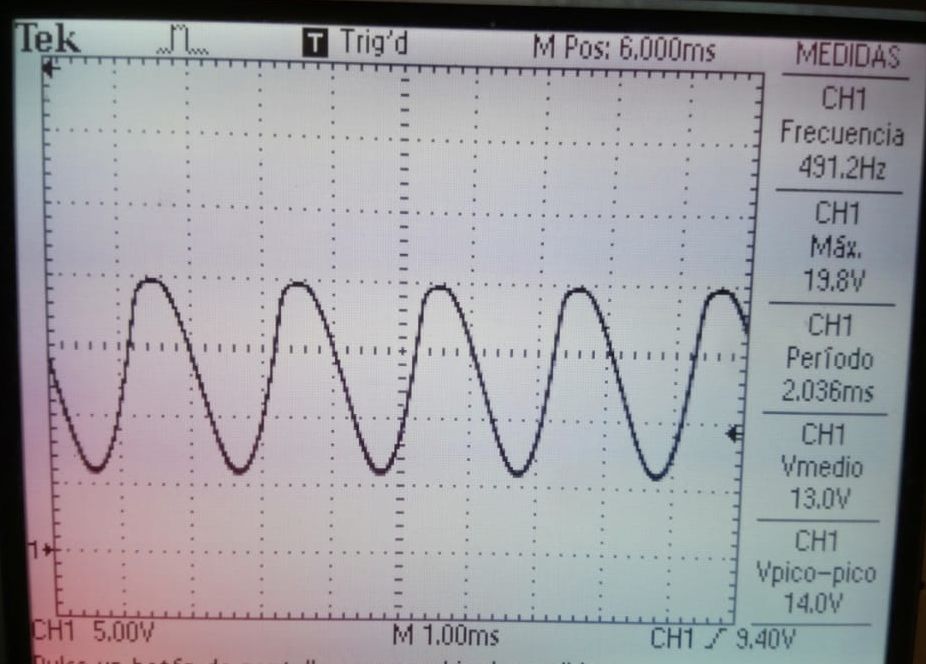
\includegraphics[width=0.5\textwidth]{med_oscilador_cc.png}
          \captionof{figure}{Simulación de la salida del oscilador.}
          \label{fig:med_out_oscilador}
        \end{center}

        \begin{center}
          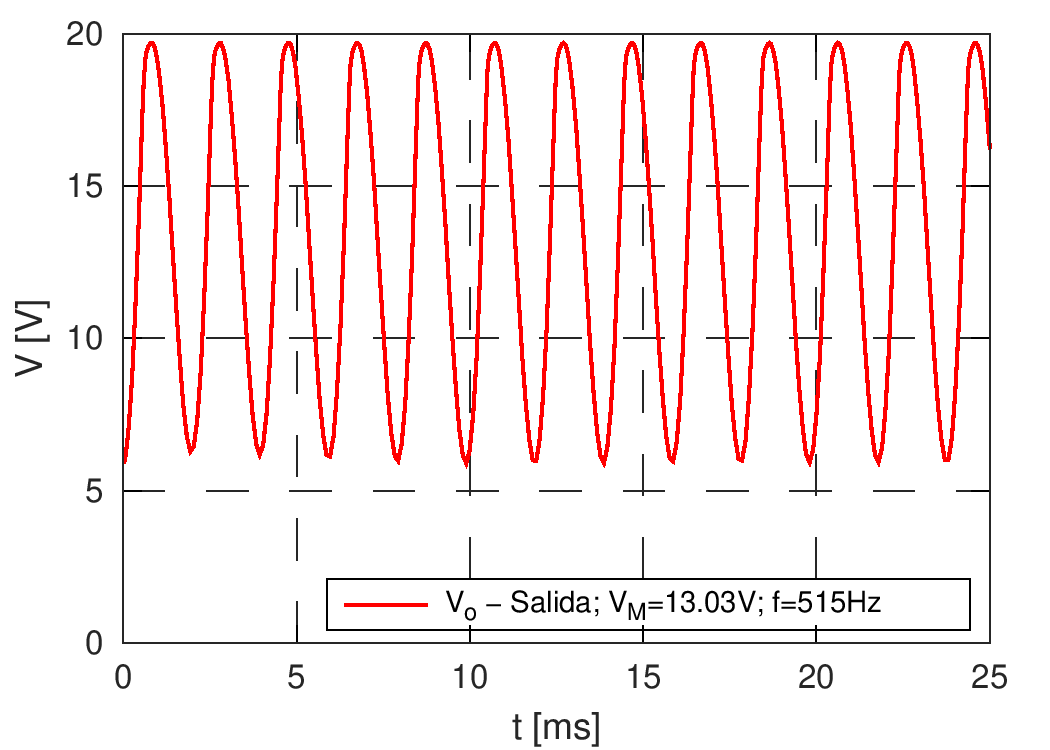
\includegraphics[width=0.5\textwidth]{salida_oscilador.png}
          \captionof{figure}{Simulación de la salida del oscilador.}
          \label{fig:sim_out_oscilador}
        \end{center}


        \begin{center}
          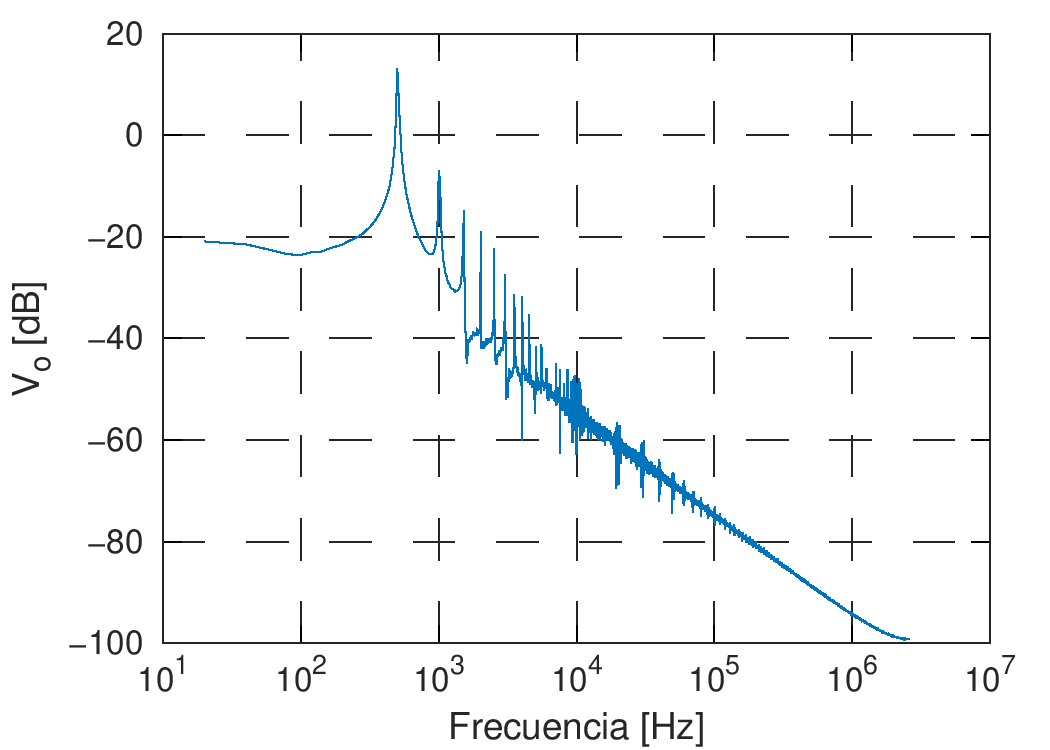
\includegraphics[width=0.5\textwidth]{fft_oscilador.png}
          \captionof{figure}{FFT de la señal de salida del oscilador obtenida mediante LTSpice.}
          \label{fig:fft}
        \end{center}


        \clearpage
                \section{Conclusiones}

        Durante la etapa amplificadora se puede notar que alcanzar una ganancia de potencia mayor a 100 es un objetivo perfectamente razonable puesto que es directamente proporcional a la ganancia de corriente, para la cual se tiene una corriente de entrada cuya magnitud es despreciable al utilizarse un FET, por lo que finalmente se regula con la resistencia de gate elegida. Por este motivo, logramos diseñar un circuito que cumple la condición propuesta. También pudimos comprobar que trabajamos en frecuencias medias para los valores elegidos. Por otro lado, en la simulación se obtuvo un valor de ganancia menor en un $85\%$ al medido en la práctica. Consideramos que esto se debe a algún parámetro no contemplado en el modelo, aunque este valor simulado también cumple la condición propuesta.

        \medskip

        Para el oscilador senoidal por desplazamiento de fase se puede destacar que inicialmente consideramos que el bloque de realimentación estaba constituido por tres bloques RC,ero para ello se requeriría que cada bloque otorgue un desfasaje de 60º, con una frecuencia asociada en el orden de los 6KHz. Dado que tanto en la simulación como en la práctica se midió una respuesta de 500Hz, se concluyó que era más coherente considerar únicamente dos bloques que desfasan 90º. Además, se pudo observar como puede detenerse el efecto de oscilación al disminuir la tensión de alimentación a un valor tal que el transistor se encuentra en corte, o con un punto Q cercano a este régimen.





        %\section{Conclusiones}

        %\section{Referencias} %Usar \printbibliography y el archivo ref.bib
        %\begin{itemize}
            %\item How Oscilloscope Probes Affect Your Measurement - Application Note - Tektronix
        %\end{itemize}
        %\printbibliography



\end{document}
